% !TEX encoding = UTF-8 Unicode
\documentclass[10pt]{standalone}\usepackage{tikz}
\usepackage{fontspec}
\setmainfont{Arial}
\setsansfont{Arial}\begin{document}

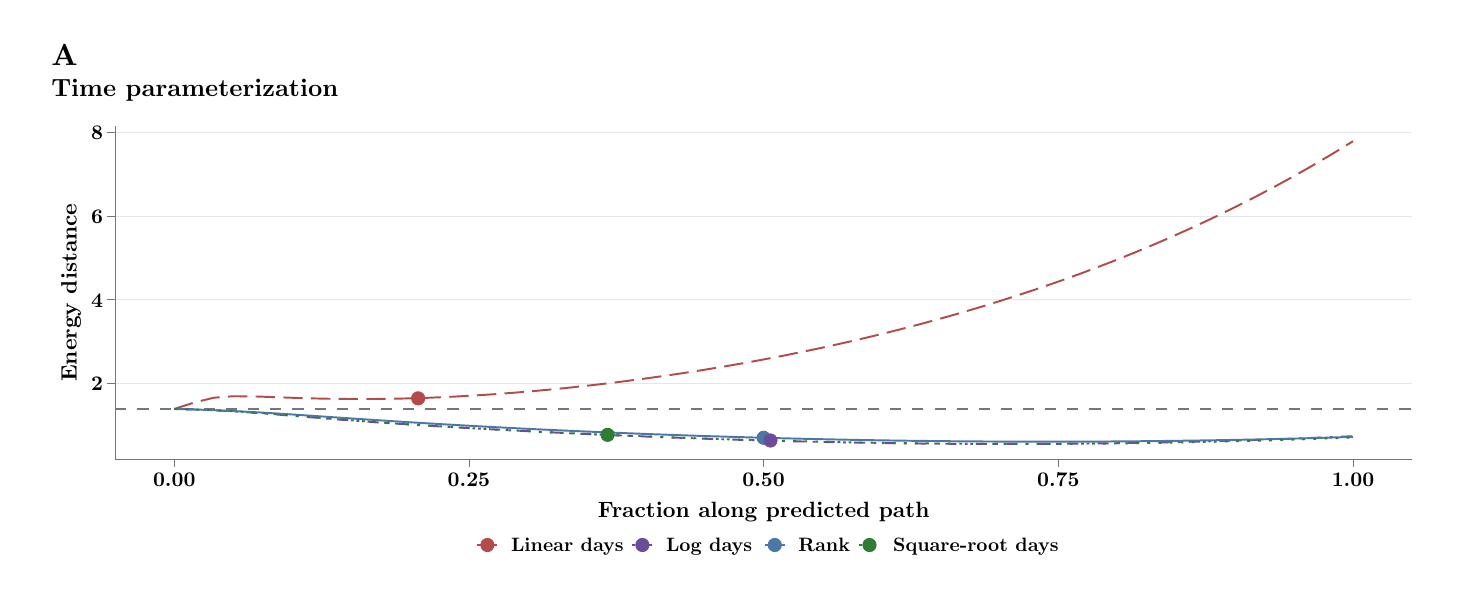
\begin{tikzpicture}[x=1pt,y=1pt]
\definecolor{fillColor}{RGB}{255,255,255}
\path[use as bounding box,fill=fillColor,fill opacity=0.00] (0,0) rectangle (512.15,199.17);
\begin{scope}
\path[clip] (  0.00,  0.00) rectangle (512.15,199.17);
\definecolor{drawColor}{RGB}{0,0,0}

\node[text=drawColor,anchor=base west,inner sep=0pt, outer sep=0pt, scale=  1.10] at (  8.54,185.60) {\bfseries A};

\node[text=drawColor,anchor=base west,inner sep=0pt, outer sep=0pt, scale=  0.90] at (  8.54,174.23) {\bfseries Time parameterization};
\end{scope}
\begin{scope}
\path[clip] (  8.54,  4.27) rectangle (503.61,168.72);
\definecolor{fillColor}{RGB}{255,255,255}

\path[fill=fillColor] (  8.54,  4.27) rectangle (503.61,168.72);
\end{scope}
\begin{scope}
\path[clip] ( 31.68, 43.27) rectangle (500.20,163.60);
\definecolor{fillColor}{RGB}{255,255,255}

\path[fill=fillColor] ( 31.68, 43.27) rectangle (500.20,163.60);
\definecolor{drawColor}{RGB}{226,231,235}

\path[draw=drawColor,line width= 0.2pt,line join=round] ( 31.68, 70.64) --
	(500.20, 70.64);

\path[draw=drawColor,line width= 0.2pt,line join=round] ( 31.68,100.89) --
	(500.20,100.89);

\path[draw=drawColor,line width= 0.2pt,line join=round] ( 31.68,131.13) --
	(500.20,131.13);

\path[draw=drawColor,line width= 0.2pt,line join=round] ( 31.68,161.38) --
	(500.20,161.38);
\definecolor{drawColor}{RGB}{115,119,123}

\path[draw=drawColor,line width= 0.4pt,dash pattern=on 4pt off 4pt ,line join=round] ( 31.68, 61.39) -- (500.20, 61.39);
\definecolor{drawColor}{RGB}{180,75,75}

\path[draw=drawColor,line width= 0.7pt,dash pattern=on 7pt off 3pt ,line join=round] ( 52.97, 61.39) --
	( 60.07, 63.68) --
	( 67.17, 65.44) --
	( 74.27, 65.99) --
	( 81.37, 65.94) --
	( 88.47, 65.69) --
	( 95.57, 65.43) --
	(102.66, 65.21) --
	(109.76, 65.06) --
	(116.86, 64.98) --
	(123.96, 64.98) --
	(131.06, 65.06) --
	(138.16, 65.22) --
	(145.26, 65.45) --
	(152.36, 65.76) --
	(159.45, 66.14) --
	(166.55, 66.58) --
	(173.65, 67.10) --
	(180.75, 67.67) --
	(187.85, 68.31) --
	(194.95, 69.01) --
	(202.05, 69.77) --
	(209.15, 70.59) --
	(216.25, 71.47) --
	(223.34, 72.41) --
	(230.44, 73.40) --
	(237.54, 74.46) --
	(244.64, 75.57) --
	(251.74, 76.74) --
	(258.84, 77.98) --
	(265.94, 79.28) --
	(273.04, 80.64) --
	(280.14, 82.07) --
	(287.23, 83.56) --
	(294.33, 85.13) --
	(301.43, 86.76) --
	(308.53, 88.47) --
	(315.63, 90.25) --
	(322.73, 92.10) --
	(329.83, 94.04) --
	(336.93, 96.05) --
	(344.02, 98.15) --
	(351.12,100.33) --
	(358.22,102.60) --
	(365.32,104.96) --
	(372.42,107.41) --
	(379.52,109.96) --
	(386.62,112.62) --
	(393.72,115.37) --
	(400.82,118.24) --
	(407.91,121.22) --
	(415.01,124.31) --
	(422.11,127.52) --
	(429.21,130.86) --
	(436.31,134.33) --
	(443.41,137.93) --
	(450.51,141.67) --
	(457.61,145.55) --
	(464.71,149.59) --
	(471.80,153.78) --
	(478.90,158.13);
\definecolor{drawColor}{RGB}{107,76,154}

\path[draw=drawColor,line width= 0.7pt,dash pattern=on 1pt off 3pt on 4pt off 3pt ,line join=round] ( 52.97, 61.39) --
	( 60.07, 61.20) --
	( 67.17, 60.92) --
	( 74.27, 60.53) --
	( 81.37, 60.05) --
	( 88.47, 59.50) --
	( 95.57, 58.93) --
	(102.66, 58.35) --
	(109.76, 57.78) --
	(116.86, 57.24) --
	(123.96, 56.72) --
	(131.06, 56.23) --
	(138.16, 55.76) --
	(145.26, 55.32) --
	(152.36, 54.89) --
	(159.45, 54.48) --
	(166.55, 54.09) --
	(173.65, 53.71) --
	(180.75, 53.35) --
	(187.85, 53.00) --
	(194.95, 52.66) --
	(202.05, 52.33) --
	(209.15, 52.02) --
	(216.25, 51.72) --
	(223.34, 51.43) --
	(230.44, 51.16) --
	(237.54, 50.90) --
	(244.64, 50.65) --
	(251.74, 50.42) --
	(258.84, 50.20) --
	(265.94, 49.99) --
	(273.04, 49.80) --
	(280.14, 49.63) --
	(287.23, 49.47) --
	(294.33, 49.32) --
	(301.43, 49.19) --
	(308.53, 49.08) --
	(315.63, 48.98) --
	(322.73, 48.90) --
	(329.83, 48.83) --
	(336.93, 48.79) --
	(344.02, 48.76) --
	(351.12, 48.74) --
	(358.22, 48.75) --
	(365.32, 48.77) --
	(372.42, 48.80) --
	(379.52, 48.86) --
	(386.62, 48.94) --
	(393.72, 49.03) --
	(400.82, 49.14) --
	(407.91, 49.27) --
	(415.01, 49.41) --
	(422.11, 49.58) --
	(429.21, 49.76) --
	(436.31, 49.96) --
	(443.41, 50.18) --
	(450.51, 50.42) --
	(457.61, 50.67) --
	(464.71, 50.95) --
	(471.80, 51.24) --
	(478.90, 51.55);
\definecolor{drawColor}{RGB}{76,120,168}

\path[draw=drawColor,line width= 0.7pt,line join=round] ( 52.97, 61.39) --
	( 60.07, 61.21) --
	( 67.17, 60.96) --
	( 74.27, 60.64) --
	( 81.37, 60.27) --
	( 88.47, 59.85) --
	( 95.57, 59.40) --
	(102.66, 58.93) --
	(109.76, 58.45) --
	(116.86, 57.97) --
	(123.96, 57.50) --
	(131.06, 57.03) --
	(138.16, 56.58) --
	(145.26, 56.15) --
	(152.36, 55.73) --
	(159.45, 55.33) --
	(166.55, 54.94) --
	(173.65, 54.57) --
	(180.75, 54.21) --
	(187.85, 53.87) --
	(194.95, 53.54) --
	(202.05, 53.23) --
	(209.15, 52.93) --
	(216.25, 52.64) --
	(223.34, 52.36) --
	(230.44, 52.10) --
	(237.54, 51.85) --
	(244.64, 51.61) --
	(251.74, 51.39) --
	(258.84, 51.18) --
	(265.94, 50.98) --
	(273.04, 50.79) --
	(280.14, 50.62) --
	(287.23, 50.46) --
	(294.33, 50.31) --
	(301.43, 50.17) --
	(308.53, 50.05) --
	(315.63, 49.94) --
	(322.73, 49.85) --
	(329.83, 49.77) --
	(336.93, 49.70) --
	(344.02, 49.65) --
	(351.12, 49.61) --
	(358.22, 49.58) --
	(365.32, 49.57) --
	(372.42, 49.57) --
	(379.52, 49.58) --
	(386.62, 49.61) --
	(393.72, 49.66) --
	(400.82, 49.72) --
	(407.91, 49.79) --
	(415.01, 49.88) --
	(422.11, 49.98) --
	(429.21, 50.09) --
	(436.31, 50.22) --
	(443.41, 50.36) --
	(450.51, 50.52) --
	(457.61, 50.69) --
	(464.71, 50.88) --
	(471.80, 51.08) --
	(478.90, 51.30);
\definecolor{drawColor}{RGB}{46,125,50}

\path[draw=drawColor,line width= 0.7pt,dash pattern=on 1pt off 3pt ,line join=round] ( 52.97, 61.39) --
	( 60.07, 61.21) --
	( 67.17, 60.95) --
	( 74.27, 60.59) --
	( 81.37, 60.13) --
	( 88.47, 59.60) --
	( 95.57, 59.02) --
	(102.66, 58.43) --
	(109.76, 57.85) --
	(116.86, 57.29) --
	(123.96, 56.76) --
	(131.06, 56.26) --
	(138.16, 55.79) --
	(145.26, 55.34) --
	(152.36, 54.90) --
	(159.45, 54.49) --
	(166.55, 54.10) --
	(173.65, 53.72) --
	(180.75, 53.35) --
	(187.85, 53.00) --
	(194.95, 52.67) --
	(202.05, 52.34) --
	(209.15, 52.04) --
	(216.25, 51.74) --
	(223.34, 51.46) --
	(230.44, 51.19) --
	(237.54, 50.94) --
	(244.64, 50.69) --
	(251.74, 50.47) --
	(258.84, 50.25) --
	(265.94, 50.05) --
	(273.04, 49.86) --
	(280.14, 49.69) --
	(287.23, 49.53) --
	(294.33, 49.39) --
	(301.43, 49.26) --
	(308.53, 49.14) --
	(315.63, 49.04) --
	(322.73, 48.96) --
	(329.83, 48.89) --
	(336.93, 48.83) --
	(344.02, 48.79) --
	(351.12, 48.76) --
	(358.22, 48.75) --
	(365.32, 48.76) --
	(372.42, 48.78) --
	(379.52, 48.82) --
	(386.62, 48.87) --
	(393.72, 48.94) --
	(400.82, 49.03) --
	(407.91, 49.13) --
	(415.01, 49.25) --
	(422.11, 49.39) --
	(429.21, 49.54) --
	(436.31, 49.71) --
	(443.41, 49.90) --
	(450.51, 50.10) --
	(457.61, 50.32) --
	(464.71, 50.56) --
	(471.80, 50.82) --
	(478.90, 51.09);
\definecolor{drawColor}{RGB}{76,120,168}
\definecolor{fillColor}{RGB}{76,120,168}

\path[draw=drawColor,line width= 0.3pt,line join=round,line cap=round,fill=fillColor] (265.94, 50.98) circle (  2.40);
\definecolor{drawColor}{RGB}{180,75,75}
\definecolor{fillColor}{RGB}{180,75,75}

\path[draw=drawColor,line width= 0.3pt,line join=round,line cap=round,fill=fillColor] (141.10, 65.22) circle (  2.40);
\definecolor{drawColor}{RGB}{46,125,50}
\definecolor{fillColor}{RGB}{46,125,50}

\path[draw=drawColor,line width= 0.3pt,line join=round,line cap=round,fill=fillColor] (209.54, 52.04) circle (  2.40);
\definecolor{drawColor}{RGB}{107,76,154}
\definecolor{fillColor}{RGB}{107,76,154}

\path[draw=drawColor,line width= 0.3pt,line join=round,line cap=round,fill=fillColor] (268.40, 49.99) circle (  2.40);
\end{scope}
\begin{scope}
\path[clip] (  0.00,  0.00) rectangle (512.15,199.17);
\definecolor{drawColor}{RGB}{115,119,123}

\path[draw=drawColor,line width= 0.3pt,line join=round,line cap=rect] ( 31.68, 43.27) --
	( 31.68,163.60);
\end{scope}
\begin{scope}
\path[clip] (  0.00,  0.00) rectangle (512.15,199.17);
\definecolor{drawColor}{RGB}{0,0,0}

\node[text=drawColor,anchor=base east,inner sep=0pt, outer sep=0pt, scale=  0.75] at ( 27.23, 67.96) {\bfseries 2};

\node[text=drawColor,anchor=base east,inner sep=0pt, outer sep=0pt, scale=  0.75] at ( 27.23, 98.20) {\bfseries 4};

\node[text=drawColor,anchor=base east,inner sep=0pt, outer sep=0pt, scale=  0.75] at ( 27.23,128.45) {\bfseries 6};

\node[text=drawColor,anchor=base east,inner sep=0pt, outer sep=0pt, scale=  0.75] at ( 27.23,158.69) {\bfseries 8};
\end{scope}
\begin{scope}
\path[clip] (  0.00,  0.00) rectangle (512.15,199.17);
\definecolor{drawColor}{RGB}{115,119,123}

\path[draw=drawColor,line width= 0.3pt,line join=round] ( 28.83, 70.64) --
	( 31.68, 70.64);

\path[draw=drawColor,line width= 0.3pt,line join=round] ( 28.83,100.89) --
	( 31.68,100.89);

\path[draw=drawColor,line width= 0.3pt,line join=round] ( 28.83,131.13) --
	( 31.68,131.13);

\path[draw=drawColor,line width= 0.3pt,line join=round] ( 28.83,161.38) --
	( 31.68,161.38);
\end{scope}
\begin{scope}
\path[clip] (  0.00,  0.00) rectangle (512.15,199.17);
\definecolor{drawColor}{RGB}{115,119,123}

\path[draw=drawColor,line width= 0.3pt,line join=round,line cap=rect] ( 31.68, 43.27) --
	(500.20, 43.27);
\end{scope}
\begin{scope}
\path[clip] (  0.00,  0.00) rectangle (512.15,199.17);
\definecolor{drawColor}{RGB}{115,119,123}

\path[draw=drawColor,line width= 0.3pt,line join=round] ( 52.97, 40.43) --
	( 52.97, 43.27);

\path[draw=drawColor,line width= 0.3pt,line join=round] (159.45, 40.43) --
	(159.45, 43.27);

\path[draw=drawColor,line width= 0.3pt,line join=round] (265.94, 40.43) --
	(265.94, 43.27);

\path[draw=drawColor,line width= 0.3pt,line join=round] (372.42, 40.43) --
	(372.42, 43.27);

\path[draw=drawColor,line width= 0.3pt,line join=round] (478.90, 40.43) --
	(478.90, 43.27);
\end{scope}
\begin{scope}
\path[clip] (  0.00,  0.00) rectangle (512.15,199.17);
\definecolor{drawColor}{RGB}{0,0,0}

\node[text=drawColor,anchor=base,inner sep=0pt, outer sep=0pt, scale=  0.75] at ( 52.97, 33.46) {\bfseries 0.00};

\node[text=drawColor,anchor=base,inner sep=0pt, outer sep=0pt, scale=  0.75] at (159.45, 33.46) {\bfseries 0.25};

\node[text=drawColor,anchor=base,inner sep=0pt, outer sep=0pt, scale=  0.75] at (265.94, 33.46) {\bfseries 0.50};

\node[text=drawColor,anchor=base,inner sep=0pt, outer sep=0pt, scale=  0.75] at (372.42, 33.46) {\bfseries 0.75};

\node[text=drawColor,anchor=base,inner sep=0pt, outer sep=0pt, scale=  0.75] at (478.90, 33.46) {\bfseries 1.00};
\end{scope}
\begin{scope}
\path[clip] (  0.00,  0.00) rectangle (512.15,199.17);
\definecolor{drawColor}{RGB}{0,0,0}

\node[text=drawColor,anchor=base,inner sep=0pt, outer sep=0pt, scale=  0.80] at (265.94, 22.17) {\bfseries Fraction along predicted path};
\end{scope}
\begin{scope}
\path[clip] (  0.00,  0.00) rectangle (512.15,199.17);
\definecolor{drawColor}{RGB}{0,0,0}

\node[text=drawColor,rotate= 90.00,anchor=base,inner sep=0pt, outer sep=0pt, scale=  0.80] at ( 17.68,103.44) {\bfseries Energy distance};
\end{scope}
\begin{scope}
\path[clip] (  0.00,  0.00) rectangle (512.15,199.17);
\definecolor{fillColor}{RGB}{255,255,255}

\path[fill=fillColor] (161.57,  7.68) rectangle (370.31, 16.79);
\end{scope}
\begin{scope}
\path[clip] (  0.00,  0.00) rectangle (512.15,199.17);
\definecolor{fillColor}{RGB}{255,255,255}

\path[fill=fillColor] (161.57,  7.68) rectangle (170.67, 16.79);
\definecolor{drawColor}{RGB}{180,75,75}

\path[draw=drawColor,line width= 0.7pt,dash pattern=on 7pt off 3pt ,line join=round] (162.48, 12.23) -- (169.76, 12.23);
\definecolor{fillColor}{RGB}{180,75,75}

\path[draw=drawColor,line width= 0.3pt,line join=round,line cap=round,fill=fillColor] (166.12, 12.23) circle (  2.40);
\end{scope}
\begin{scope}
\path[clip] (  0.00,  0.00) rectangle (512.15,199.17);
\definecolor{fillColor}{RGB}{255,255,255}

\path[fill=fillColor] (217.58,  7.68) rectangle (226.68, 16.79);
\definecolor{drawColor}{RGB}{107,76,154}

\path[draw=drawColor,line width= 0.7pt,dash pattern=on 1pt off 3pt on 4pt off 3pt ,line join=round] (218.49, 12.23) -- (225.77, 12.23);
\definecolor{fillColor}{RGB}{107,76,154}

\path[draw=drawColor,line width= 0.3pt,line join=round,line cap=round,fill=fillColor] (222.13, 12.23) circle (  2.40);
\end{scope}
\begin{scope}
\path[clip] (  0.00,  0.00) rectangle (512.15,199.17);
\definecolor{fillColor}{RGB}{255,255,255}

\path[fill=fillColor] (265.41,  7.68) rectangle (274.52, 16.79);
\definecolor{drawColor}{RGB}{76,120,168}

\path[draw=drawColor,line width= 0.7pt,line join=round] (266.32, 12.23) -- (273.61, 12.23);
\definecolor{fillColor}{RGB}{76,120,168}

\path[draw=drawColor,line width= 0.3pt,line join=round,line cap=round,fill=fillColor] (269.96, 12.23) circle (  2.40);
\end{scope}
\begin{scope}
\path[clip] (  0.00,  0.00) rectangle (512.15,199.17);
\definecolor{fillColor}{RGB}{255,255,255}

\path[fill=fillColor] (299.63,  7.68) rectangle (308.74, 16.79);
\definecolor{drawColor}{RGB}{46,125,50}

\path[draw=drawColor,line width= 0.7pt,dash pattern=on 1pt off 3pt ,line join=round] (300.54, 12.23) -- (307.83, 12.23);
\definecolor{fillColor}{RGB}{46,125,50}

\path[draw=drawColor,line width= 0.3pt,line join=round,line cap=round,fill=fillColor] (304.19, 12.23) circle (  2.40);
\end{scope}
\begin{scope}
\path[clip] (  0.00,  0.00) rectangle (512.15,199.17);
\definecolor{drawColor}{RGB}{0,0,0}

\node[text=drawColor,anchor=base west,inner sep=0pt, outer sep=0pt, scale=  0.70] at (174.67,  9.73) {\bfseries Linear days};
\end{scope}
\begin{scope}
\path[clip] (  0.00,  0.00) rectangle (512.15,199.17);
\definecolor{drawColor}{RGB}{0,0,0}

\node[text=drawColor,anchor=base west,inner sep=0pt, outer sep=0pt, scale=  0.70] at (230.68,  9.73) {\bfseries Log days};
\end{scope}
\begin{scope}
\path[clip] (  0.00,  0.00) rectangle (512.15,199.17);
\definecolor{drawColor}{RGB}{0,0,0}

\node[text=drawColor,anchor=base west,inner sep=0pt, outer sep=0pt, scale=  0.70] at (278.52,  9.73) {\bfseries Rank};
\end{scope}
\begin{scope}
\path[clip] (  0.00,  0.00) rectangle (512.15,199.17);
\definecolor{drawColor}{RGB}{0,0,0}

\node[text=drawColor,anchor=base west,inner sep=0pt, outer sep=0pt, scale=  0.70] at (312.74,  9.73) {\bfseries Square-root days};
\end{scope}
\end{tikzpicture}

\end{document}
